% this file is called up by thesis.tex
% content in this file will be fed into the main document

\chapter{Recommendations} % top level followed by section, subsection
\label{cha:rec}

% ----------------------- contents from here ------------------------
%

This chapter presents practical recommendations for the readers who
wish to use the new data processing pipeline presented in this report.
The chapter also presents alternative paths of research which remain
unexplored and general improvements that can be made to the pipeline
in the future.

\section{On the MLP}
The Multi Layer Perceptron presented in Chapter \ref{cha:mlp} is
capable of identifying causally related hits with a higher accuracy,
precision and recall compared to the Pattern Matrix Criterion
presented by Karas et al. (2019). It is therefore considered a viable
successor to the PMC. Although experiments were done to identify the
optimal parameters such as the batch size, optimization function,
learning rate, height and depth of the network, further
experimentation is recommended before it is integrated into the Data
Acquisition Pipeline. The model also showed an increase in the number
of FPs when the number of positive class examples increased. It may be
possible to correct this bias by adding some regularization into the
model \cite{goodfellow2016deep}.

\begin{table}[htb]
  \centering
  \caption{Advanced edge weight scheme for GCN.}
  \begin{tabular}{lr}
    \hline
    Node type(s) & Edge weight \\
    \hline
    noise-noise & 1.0 \\
    event-event (causally related) & 1.0 \\
    event-event (causally unrelated) & 0.5 \\
    event-noise & 0.1 \\
    \hline
  \end{tabular}
  \label{tab:gcn-adv-weights}
\end{table}

\section{On the GCN}
The GCN obtained in Chapter \ref{cha:gcn} has a perfect recall however
is also significantly biased to the positive class (event nodes) and
thus unable to identify the negative class (noise nodes). The origin
of the problem can be traced back to the edge weights being applied to
the graph. The weights supplied by the MLP only take into account
edges between causally related and unrelated hits. In reality however,
unrelated hits consists of various sub categories: 1. noise-noise hits
2. noise-event hits and 3. causally unrelated event-event hits.
Although from a physics point of view the pairs of hits listed above
are in fact causally unrelated, this \emph{naive} edge weight scheme
does not allow the GCN to learn adequately. The root cause of this
conflict is based in the fact that the two models have contradictory
goals. Whilst the MLP is trained to identify causally related and
unrelated hits, the GCN is required to identify hits originating from
neutrino events and noise. The solution is simple and requires
assigning edge weights based on the nodes that it connects as
summarized in Table \ref{tab:gcn-adv-weights}. The GCN model is
trained using the \emph{advanced} edge weight scheme and the results
are promising as observed in Figure \ref{fig:gcn-cm-adv} and
\ref{fig:gcn-test-tsne-adv}. The model now has perfect discriminatory
skills for both classes even in the extremely skewed datasets like
TS2.

\begin{figure}[htb]
  \centering
  \subfloat[TS1 after.]{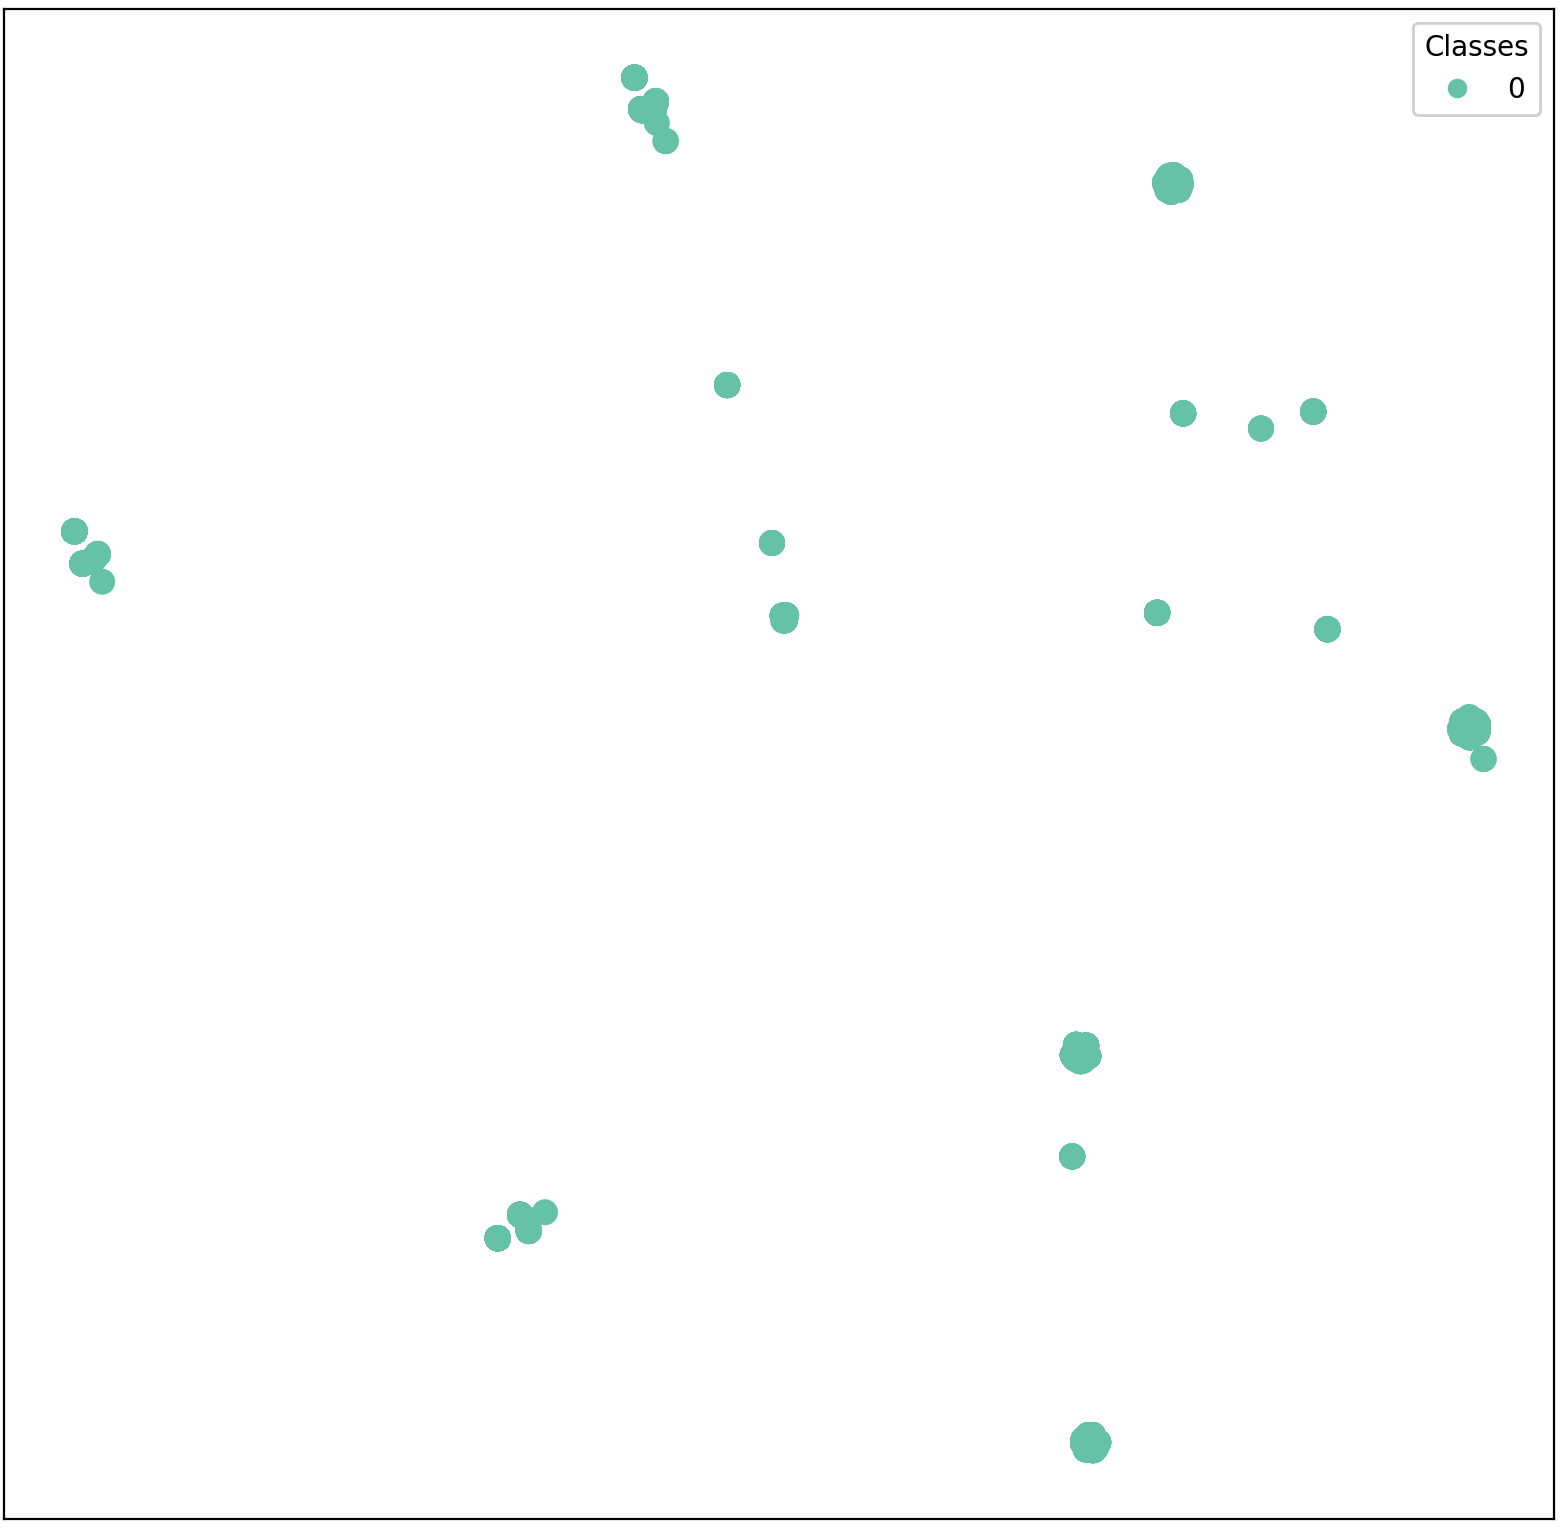
\includegraphics[width=0.33\textwidth]{gcd-adv-test-no-tsne-after.png}}
  \subfloat[TS2 after.]{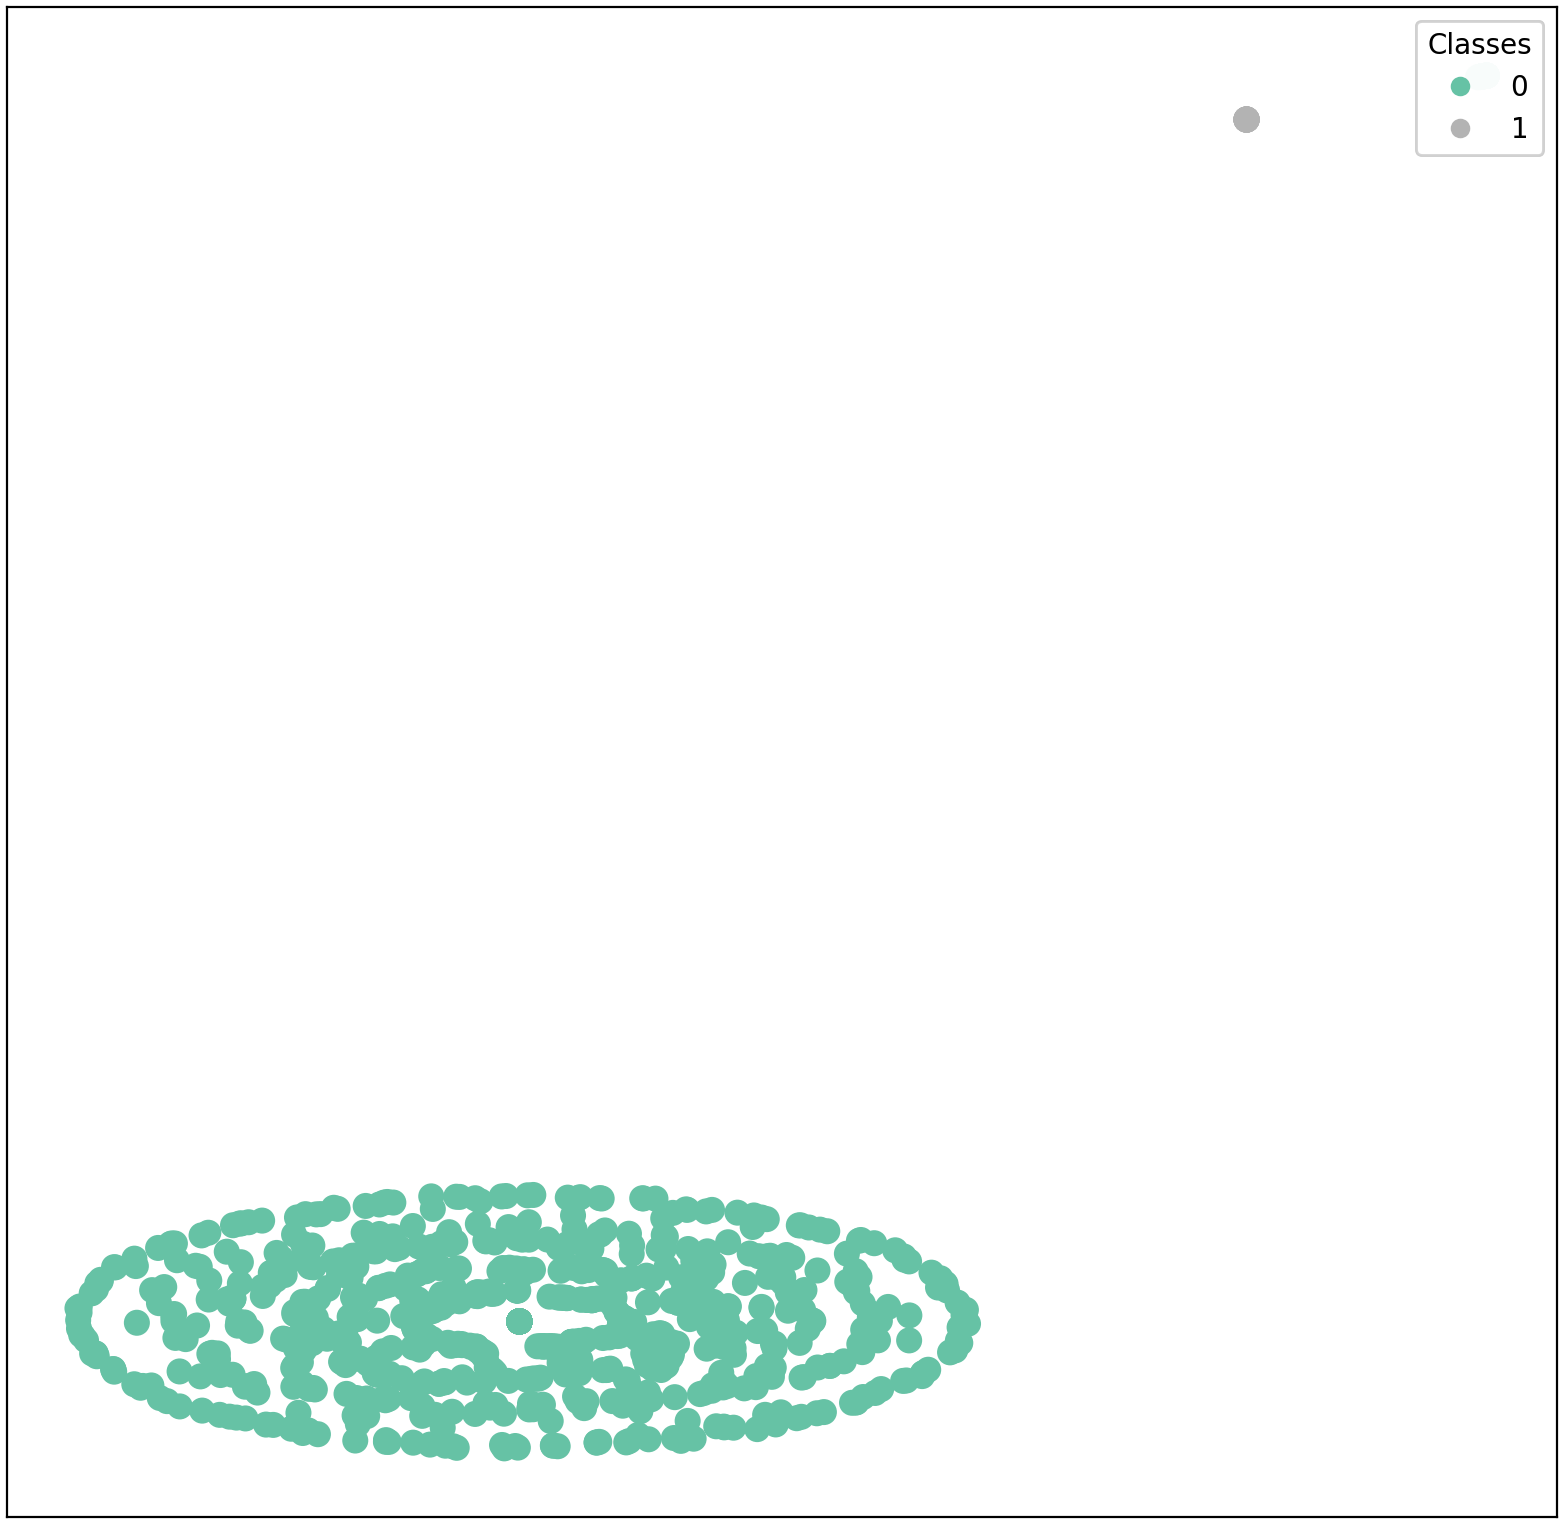
\includegraphics[width=0.33\textwidth]{gcd-adv-test-medium-tsne-after.png}}
  \subfloat[TS3 after.]{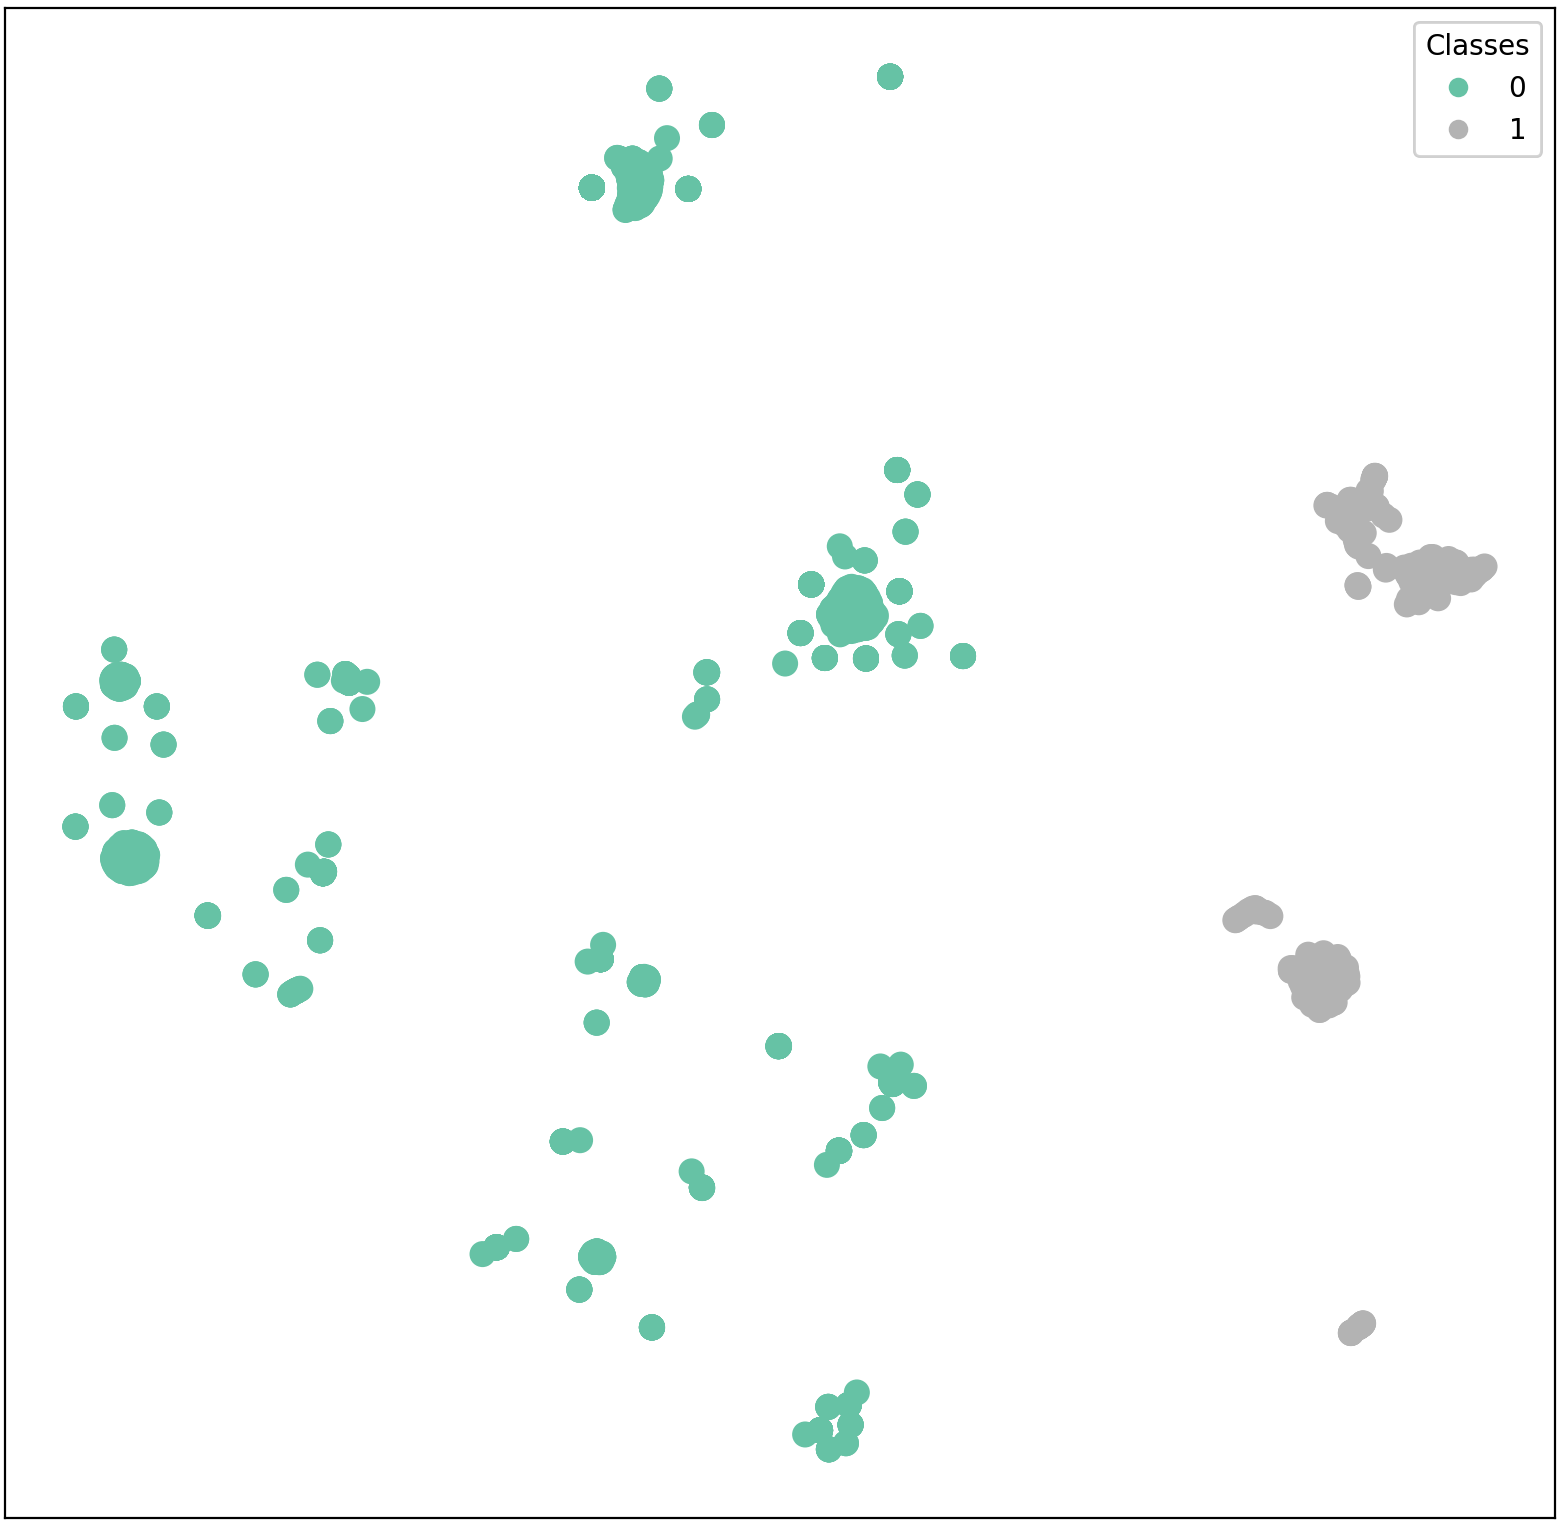
\includegraphics[width=0.33\textwidth]{gcd-adv-test-high-tsne-after.png}}
  \caption{TSNE for GCN test datasets with advanced edge weights.}
  \label{fig:gcn-test-tsne-adv}
\end{figure}

\begin{figure}[htb]
  \centering
  \subfloat[CM for TS1.]{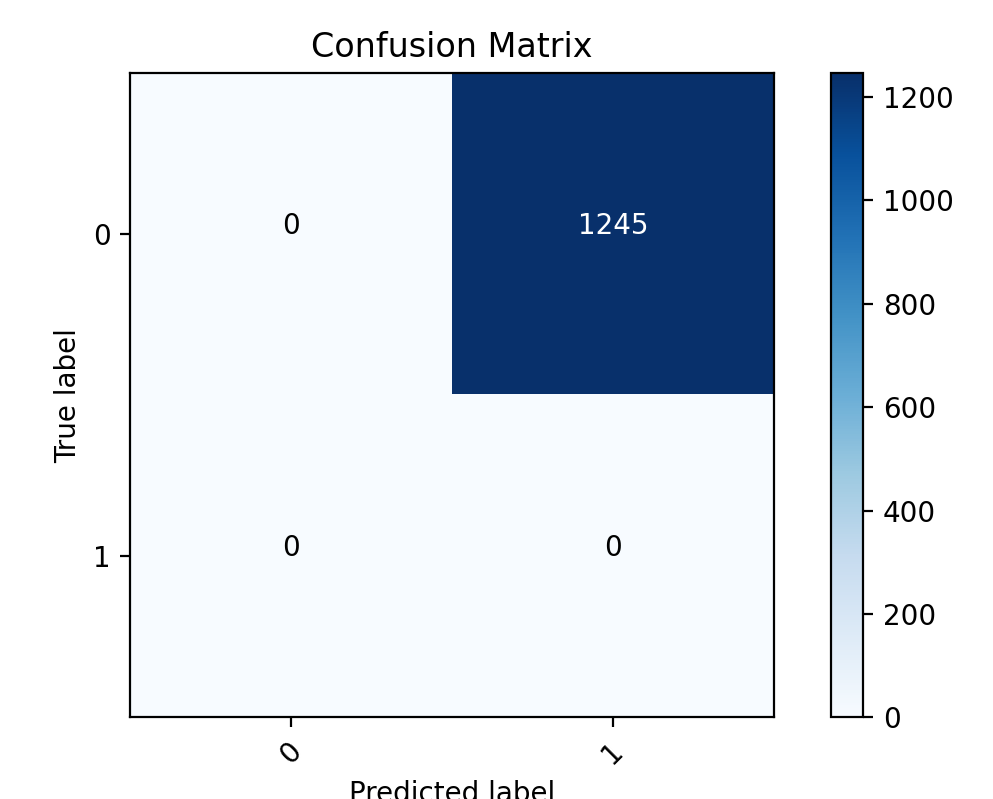
\includegraphics[width=0.33\textwidth]{gcd-adv-cm-no.png}}
  \subfloat[CM for TS2.]{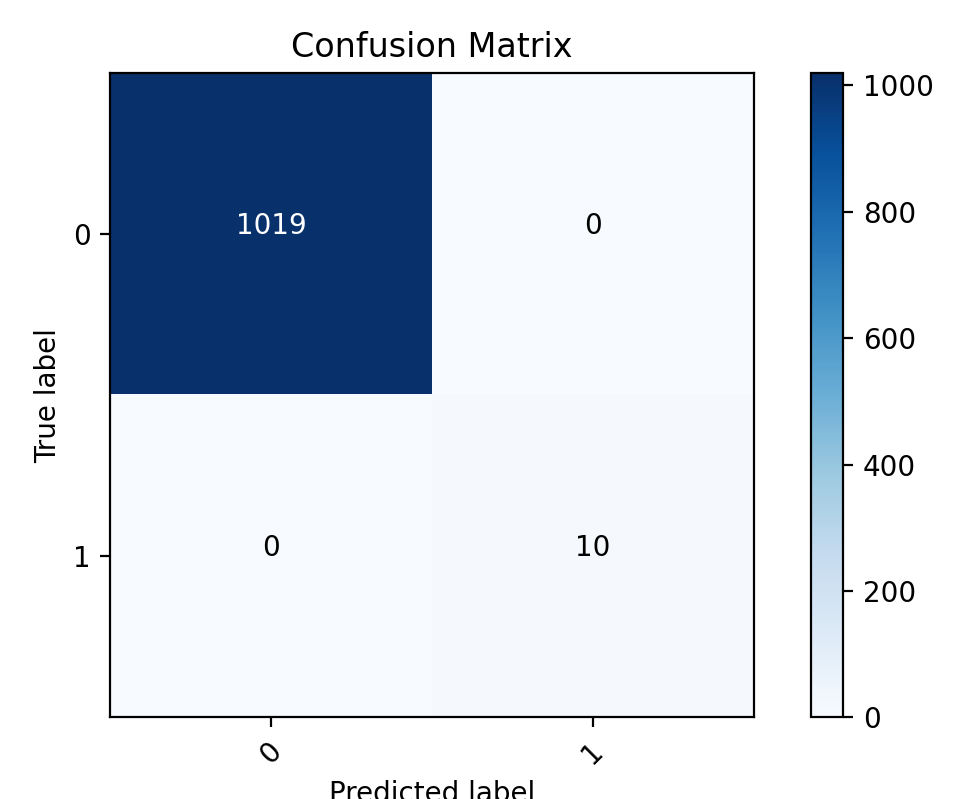
\includegraphics[width=0.33\textwidth]{gcd-adv-cm-medium.png}}
  \subfloat[CM for TS3.]{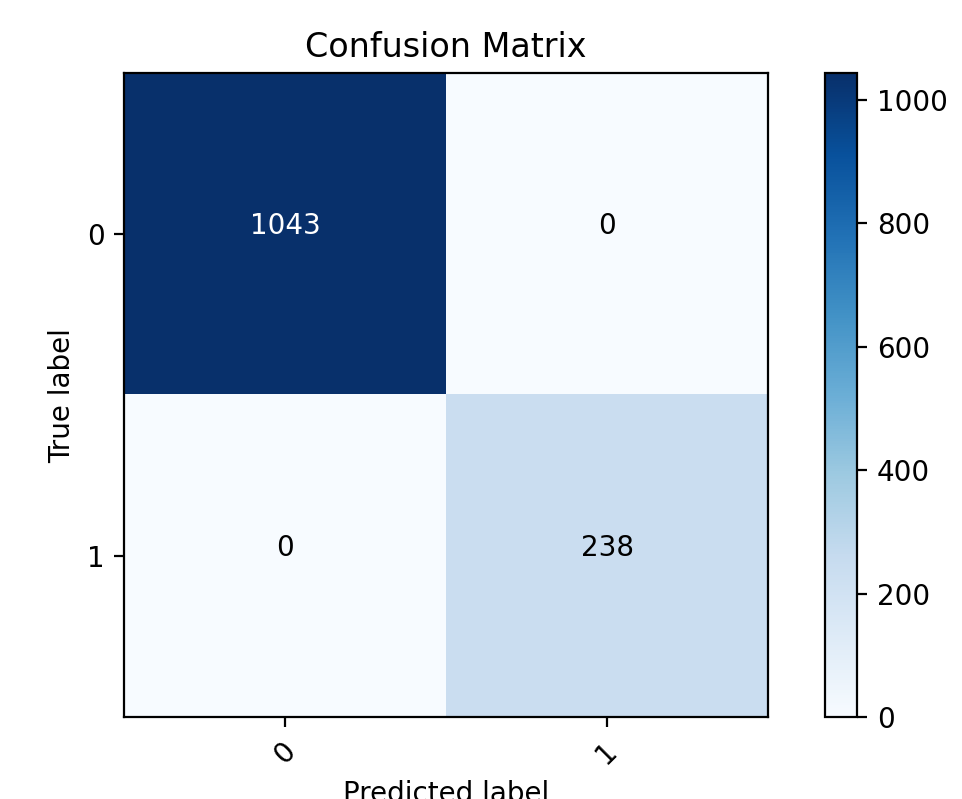
\includegraphics[width=0.33\textwidth]{gcd-adv-cm-high.png}}
  \caption{CM for GCN test datasets with advanced edge weights.}
  \label{fig:gcn-cm-adv}
\end{figure}

Although the GCN is now capable of identifying event and noise nodes
with immaculate accuracy, precision and recall, it however classifies
all examples as false positives in TS1 which contains no event nodes.
The model is impeded by the high weights on edges between causally
related event nodes and noise nodes, which may be corrected by framing
the data as a multi-edge heterogeneous graph. By creating different
types of edges corresponding to the various types of connections that
two nodes may posses, each carrying the corresponding weights, the
network may be able to correct its bias to the positive class. In
order to obtain the advanced edge weight, the MLP must be modified
such that it performs multi-class classification on the edge types.
For a classification problem of n edge types, the output of the MLP
will thus become a \texttt{(n,)} vector containing the expected
probability for each class. These probabilities can then be used as
the edge weights. The MLP may not be able to discern causally
unrelated hits since they are spread evenly in space and time. Thus
research to identify an appropriate model for the task is required.
One such approach may be to use a GCN to perform classification of the
edge types or regression on the edge weights
\cite{gong2019exploiting}.

\begin{table}[htb]
  \centering
  \caption{Summary of GCN performance across test sets with advanced
    edge weights.}
  \begin{tabular}{lrrrrrrr}
    \hline
    & Accuracy & Precision & Recall & F1 & F2 & ROCAUC & PRAUC \\
    \hline
    \textbf{TS1} & 0.00 & -- & -- & -- & -- & -- & -- \\
    \textbf{TS2} & 1.00 & 1.00 & 1.00 & 1.00 & 1.00 & 1.00 & 1.00 \\
    \textbf{TS3} & 1.00 & 1.00 & 1.00 & 1.00 & 1.00 & 1.00 & 1.00 \\
    \hline
  \end{tabular}
  \label{tab:gcn-results-adv}
\end{table}

\section{On Independence of the Models}

\begin{figure}[htb]
  \centering
  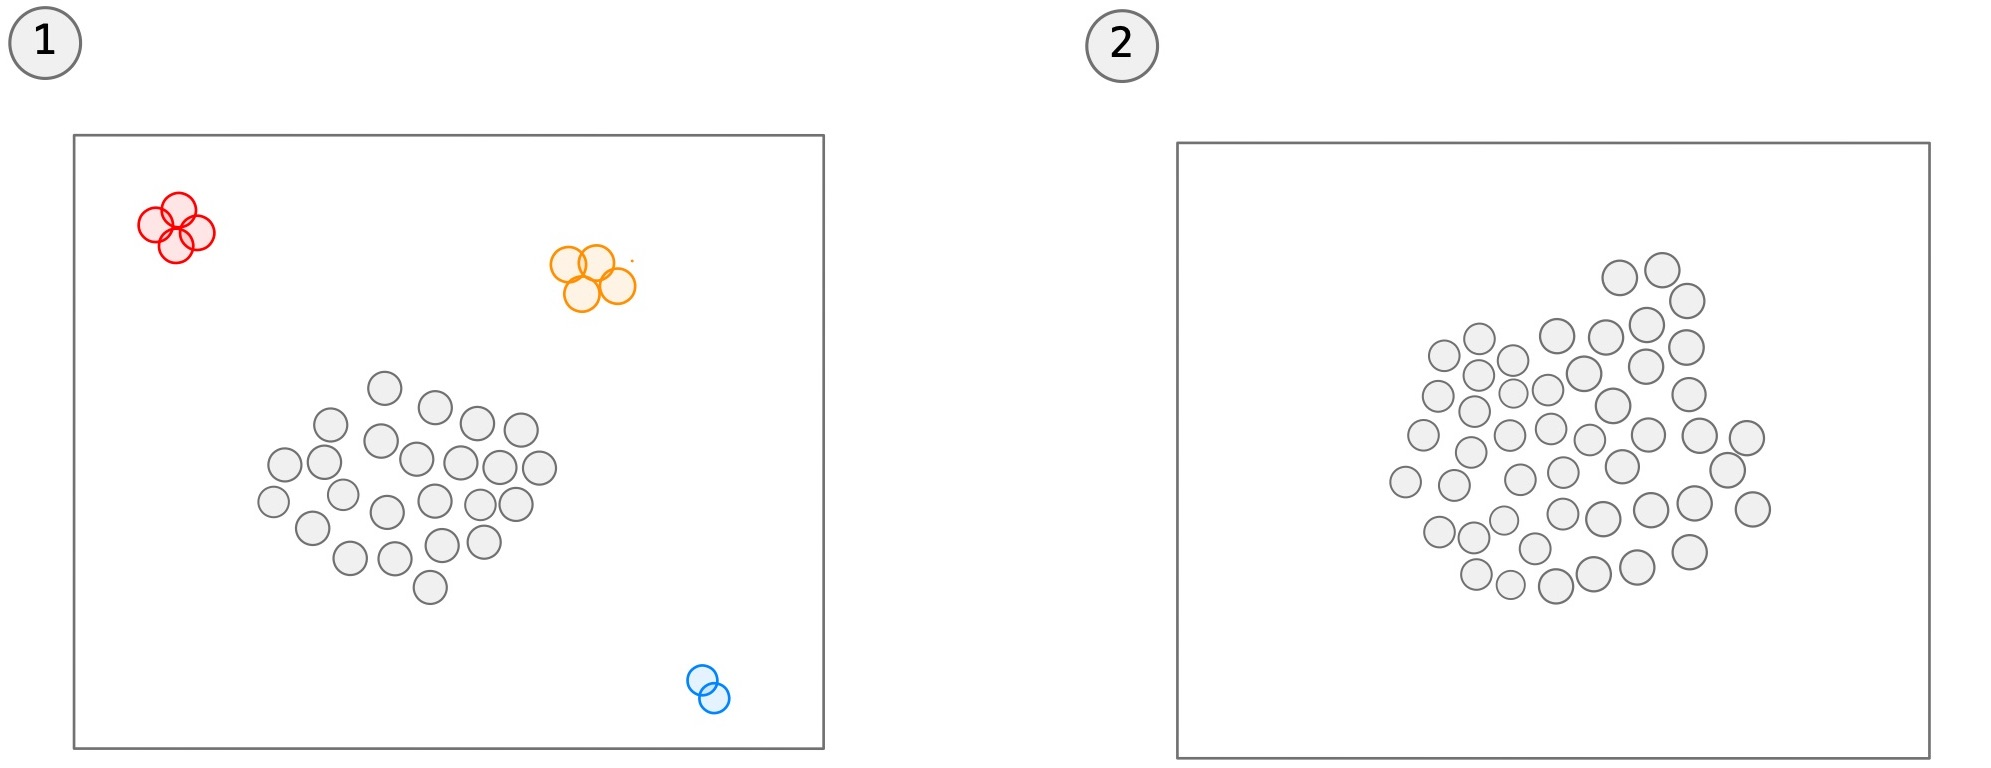
\includegraphics[width=\textwidth]{gcn-ind.jpg}
  \caption{Illustration of a possible training set for the graph
    classification model.}
  \label{fig:gcn-ind}
\end{figure}
      
There is a high dependency on the Hit Correlation Step by the
subsequent steps of the GPU Pipeline. The output of the PMC is used by
these subsequent steps so any shortcomings of the PMC cascade down
affecting the performance of the latter steps and the pipeline as a
whole. This dependency is also present in the new pipeline as the
performance of the MLP directly dictates the performance of the GCN.
This dependency is not ideal and an effective solution to make the
models independent is required. One such solution is to explore the
possibility of replacing the entire pipeline with a single GCN. The
data can be framed such that the $(x, y, z)$ vectors are used as the
node embedding. If the \emph{t} is scaled between $[0, 1]$ and the
complement of $\Delta t$ is assigned as the edge weights, it should
result in a graph where edges between causally related nodes carry a
high weight. After convolusion, a reasonable expectation is the
presence of small and tightly connected communities of causally
related nodes and large, weakly connected communities of noise nodes
(illustrated in Figure \ref{fig:gcn-ind}). The GCN model can now be
modified to perform graph classification \cite{zhang2018end} instead
of node classification. The premise being that presence of small,
densely connected communities indicate the timeslice is important and
thus should be saved for further analysis. Alternatively, the Line
Graph Neural Network proposed by Chen et al. (2017) built specifically
for community detection can also be used.

\section{On the Runtime Performance}
The models presented in this report were tested in isolation. The
intended usage however is to use them in tandem in order to identify
timeslices containing neutrino event hits. Thus it is recommended that
the models be tested as an integrated pipeline so that the results may
be compared to that of the GPU Pipeline. Additionally, performance of
the pipeline should be observed using various permutations of the
individual parts of the new and the old pipeline to determine the best
performing combination overall. As noted in Section
\ref{sec:user-req}, the runtime performance of the pipeline is crucial
and should be able to perform filtration in near real time. As neural
networks can be parallelized using the compute power of GPUs, the
models should be capable of meeting the requirements. Several existing
work also indicate the feasibility of scaling GCNs to parallel
computation over large graphs \cite{ma2019high, ma2019neugraph,
  zeng2019accurate}. However the data preparation for the models
presented in Section \ref{sec:mlp-data-prep} and
\ref{sec:gcn-data-prep} may pose a bottleneck since they are not
instantaneous. Of course at this point these are merely speculations
and empirical proof still requires to be gathered.

% ---------------------------------------------------------------------------
% ----------------------- end of thesis sub-document ------------------------
% ---------------------------------------------------------------------------
